
\section{Introduction}

Capacitors with high energy and power are essential for efficient management of electrical power.  Order of magnitude increases are desired for energy and power density. This may be possible with new self-repairing titanate dielectric capacitors using high surface area doped titanium and doped zirconium-titanium.  Anodizing at DC voltages forms a uniform dielectric film of doped titanium (the energy density of this dielectric is estimated to be on the order of 150J/$cm^3$) \cite{tiSponge}. This and the volume fraction of dielectric determines the energy density of the capacitor.

One of the major problems plaguing titanium electrolytic capacitors has been their high leakage currents \cite{tiCharHag}. In order to further research into titanium capacitors, custom anodization instrumentation has been developed to anodize and characterize a large number of candidate titanium capacitor materials. This instrumentation was necessary because conventional systems do not have the necessary dynamic range (1A-1nA measurement) or repeatability needed in this application.


\subsection{Anodization Process and Requirements}

%Anodization is the act of growing an oxide layer (dielectric) on top of a metal anode. Dielectrics are benificial because they allow capacitors to store more energy for a given electric field \cite{cwruEncDie}. The anodization process is preformed by connecting a voltage or current source to an anode and a cathode and immersing them in an electrolyte solution as shown in Fig. ~\ref{fig:anodSetup}

\begin{figure}[here]
\centering
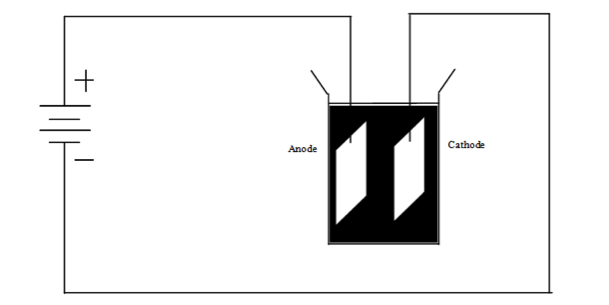
\includegraphics{anodSetup}
\caption{Anodization Setup}
\label{fig:anodSetup}
\end{figure}


Referring to Fig. ~\ref{fig:anodSetup}, in the simplest case, the current transfer is an ionic transfer where the Ti anode reacts with $O_{2}$ to create a $TiO_{2}$ oxide layer. The reaction at the metal-oxide surface can be written as:

\begin{equation}
Ti + 0_2 => TiO_2 + 4e
\end{equation}
The titanium also reacts with the electrolyte solution to give off hydrogen:
\begin{equation}
Ti + 2H_20 => Ti0_2 + 4H+Ti0_2
\end{equation}
This hydrogen reacts with the electrons at the cathode to create hydrogen gas and complete the ionic circuit.
\begin{equation}
4H + 4e => 2H_20
\end{equation}

This process is very similar to anodizing aluminum. For an explanation of that process visit \cite{cwruEncAlanod}.

Since the rate of oxide formation is dependent on the charge transport into the anode during anodization \cite{tiMinit}, a current source was selected. A typical anodization process with a current source will see the current and voltage progress as in Fig. ~\ref{fig:anodCurve}.


\begin{figure}[here]
\centering
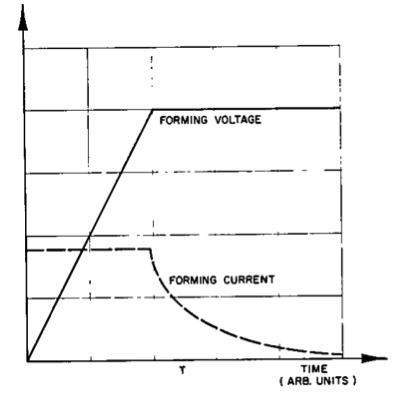
\includegraphics{anodCurve}
\caption{Anodization Curve \cite{tiMinit}}
\label{fig:anodCurve}
\end{figure}

Our typical anodization tests work with a constant current of 20mA and a forming voltage of 30V. The anodization reaches the forming voltage in periods on the order of 30 seconds. The forming voltage then remains constant while the leakage current decreases over  a much longer time period (on the order of 24 hours) to currents on the order of 1 uA or less. The exact times and values are dependent upon the material and the size of the electrode.

If a constant current is introduced, the voltage will (ideally) rise linearly with time. This will happen until the anode reaches the compliance voltage, at which point the current through the DUT will begin to drop off until it reaches the leakage current of the unpackaged capacitor. 
